% Number 890
% CAPMG  Units 
% Graphs modeling motion
% KO

% Watermark
\AddToShipoutPicture*{\BackgroundPic}

\addtocounter {ProbNum} {1}

%\begin{floatingfigure}[r]{.44\textwidth}
%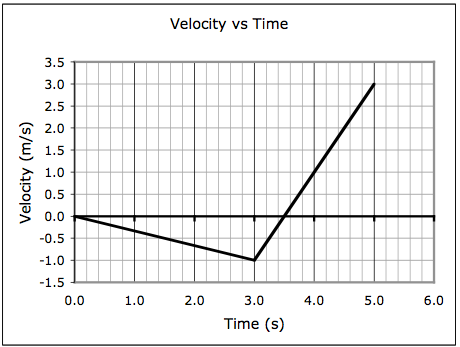
\includegraphics[scale=.54]{/Users/jgates/desktop/latex/pics/vgraph6}
%\end{floatingfigure}
 
{\bf \Large{\arabic{ProbNum}}} For each of the following motions, draw a position graph and a velocity graph (with accurate numbers on the axes). Define up/right positive, down/left negative. As always, state any assumptions that you make.\bigskip

A car starts from rest, steadily speeds up to ${30~\tfrac{m}{s}}$ in 15 seconds, moves at a constant speed for 30 seconds, then comes to a halt in 5 seconds.
\vfill

A rock is dropped from a bridge and steadily speeds up as it falls. It is moving at ${30~\tfrac{m}{s}}$ three seconds later, when it hits the ground.

\vfill

%\begin{center}
%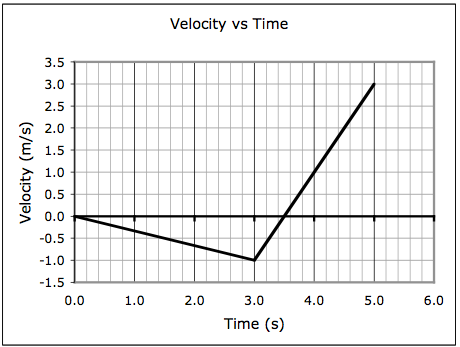
\includegraphics[scale=1]{/Users/jgates/desktop/latex/pics/vgraph6}
%\end{center}


\newpage